% ============================================================================
%  Benchmarking salarial - presentacion de defensa
%
%  COMPILAR:  pdflatex presentacion.tex   (dos veces)
%
%  PLANTILLA: pmichaillat/latex-presentation (MIT). `presentation.sty` esta
%  vendorizado sin modificar junto a este fichero, con su licencia en
%  `presentation-LICENSE.md`. La plantilla espera las figuras en un solo PDF
%  multipagina; aqui se usan los cuatro PDF sueltos que ya emite `figuras.py`,
%  que es lo unico que se aparta de ella.
%
%  Cifras: `docs/mediciones.md` y `docs/registro_decisiones.md`. Las mismas que
%  las de `tesis.tex`.
% ============================================================================
\documentclass[11pt, xcolor={dvipsnames}, usepdftitle=false]{beamer}
\usepackage{presentation}

% `es-noshorthands` desactiva los atajos de babel (`~n`, `"a`), que en beamer
% chocan con los overlays; `es-nolists` deja el espaciado de listas al tema.
\usepackage[spanish, es-noshorthands, es-nolists, es-tabla]{babel}

\graphicspath{{figuras/}}

\hypersetup{pdfpagemode=UseNone, hidelinks, pdfdisplaydoctitle=true,
pdftitle={Benchmarking salarial con etiquetas de puesto delgadas}}

\newcommand{\cargo}[1]{\texttt{\small #1}}

\title{Benchmarking salarial con etiquetas de puesto delgadas}
\author{Pablo Andrés Encalada}
\date{Maestría en Inteligencia Artificial, USFQ}

\begin{document}
\frame{\titlepage}

% ----------------------------------------------------------------------------
\begin{frame}
\frametitle{El problema está en el condicionante, no en el estimador}
\begin{itemize}
\item Un benchmark salarial estima cuantiles de la distribución de sueldos
condicionada al puesto. El estimador es una mediana ponderada; la especificación
del condicionante es el problema abierto.
\item La práctica establecida impone una taxonomía cerrada y traslada el mapeo al
cliente. Ese mapeo es manual, no reproducible entre codificadores, y su tasa de
acuerdo no se publica.
\item Aquí se usa la etiqueta de cargo declarada por el empleador, en texto
libre, y se mide cuánto del error es atribuible a agrupar mal.
\end{itemize}
\vspace{3mm}
Datos: estudios actuariales de nómina, Ecuador, 2024--2025, cruzados con el
registro de la Superintendencia de Compañías.
\end{frame}

% ----------------------------------------------------------------------------
\begin{frame}
\frametitle{El catálogo de cargos está en régimen de área pequeña}
\begin{columns}[T]
\begin{column}{0.42\textwidth}
\vspace{6mm}
\begin{tabular*}{\textwidth}{@{\extracolsep\fill}lr}
\toprule
Títulos distintos & 65.181 \\
Personas por título & 2 \\
Empresas por título & 1 \\
\bottomrule
\end{tabular*}
\vspace{2mm}
{\footnotesize Las dos últimas filas son medianas.}

\vspace{5mm}
El \al{78\,\%} de los títulos tiene una sola empresa y cubre el 21\,\% de las
personas. El 1\,\% con 30 o más empresas cubre el 46\,\%.
\end{column}
\begin{column}{0.56\textwidth}
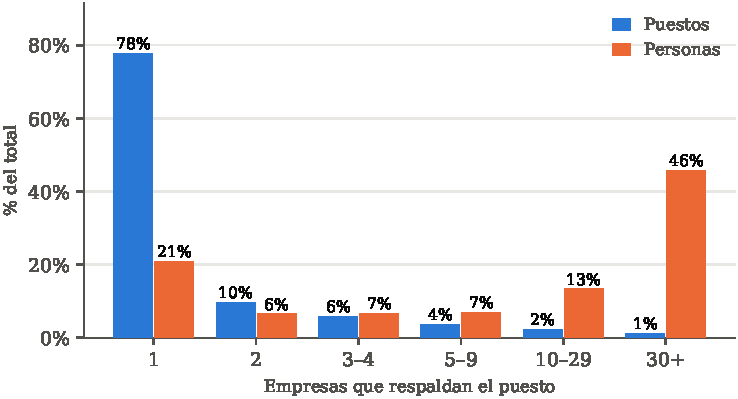
\includegraphics[width=\textwidth]{espesor_catalogo.pdf}
\end{column}
\end{columns}
\vspace{2mm}
La mayoría de las celdas no admite estimación directa. El problema es de
estimación en áreas pequeñas, no de clasificación.
\end{frame}

% ----------------------------------------------------------------------------
\begin{frame}
\frametitle{El error irreducible acota la ganancia disponible}
Con $y = \log(\text{sueldo}/\text{SBU})$, dentro de cada celda de cargo $c$:
\[
y_{fi} = \mu_c + u_f + e_{fi}, \qquad
u_f \sim (0, \tau^2), \qquad e_{fi} \sim (0, \sigma^2).
\]
\begin{columns}[T]
\begin{column}{0.44\textwidth}
Sobre el ajuste, $\tau = 0{,}2917$ y $\sigma = 0{,}1423$: el efecto empleador
explica el \al{81\,\%} de la varianza residual.

\vspace{3mm}
Contra ese suelo, el techo de mejora por reagrupar es del \al{12,1\,\%}, y del
13,2\,\% sin la censura del SBU. Es la referencia del trabajo, no el cero.
\end{column}
\begin{column}{0.54\textwidth}
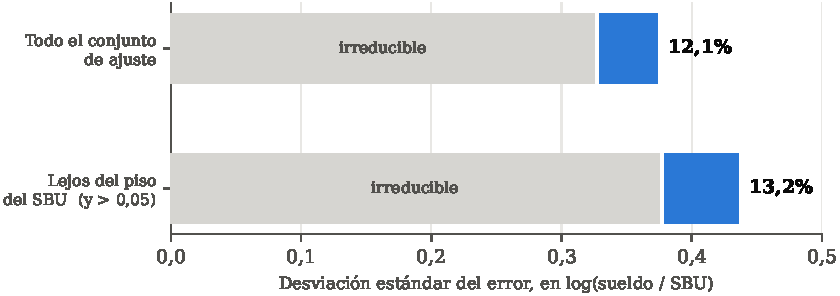
\includegraphics[width=0.96\textwidth]{descomposicion_error.pdf}
\end{column}
\end{columns}
\end{frame}

% ----------------------------------------------------------------------------
\begin{frame}
\frametitle{Estimador: cuantil ponderado por inverso de varianza}
El voto de la empresa $f$ es la mediana de sus $n_f$ personas en la celda. La
referencia es el cuantil ponderado al 50\,\% de los votos, con
\[
w_f = \frac{1}{\tau_c^2 + \sigma_c^2/n_f}.
\]
\begin{itemize}
\item Los dos regímenes límite son las dos convenciones del campo:
$n_f \to \infty$ da $w_f \to 1/\tau_c^2$, un voto por empresa; $\tau_c^2 \to 0$
da $w_f \to n_f/\sigma_c^2$, un voto por persona.
\item El ratio de pesos está acotado por la razón de varianzas,
$w_{\max}/w_{\min} \le 1 + \sigma_c^2/\tau_c^2 \approx \al{1{,}24}$, no por el
tamaño relativo de las empresas. No hace falta truncar el voto de las grandes.
\item $\tau_c$ y $\sigma_c$ se estiman por celda. El estimador no tiene
hiperparámetros.
\end{itemize}
\end{frame}

% ----------------------------------------------------------------------------
\begin{frame}
\frametitle{Vecindario semántico: la similitud no es el peso}
Ponderar los vecinos por similitud $\times$ precisión invierte el orden correcto:
\vspace{2mm}
\begin{tabular*}{\textwidth}{@{\extracolsep\fill}lrr}
\toprule
Vecinos de \cargo{OPERADOR DE PARQUEADERO} & Similitud & Peso \\
\midrule
\cargo{OPERADOR DE PARQUEADEROS} & 0,989 & 8\,\% \\
\cargo{OPERADOR DE EXCAVADORA} & 0,825 & \al{46\,\%} \\
\bottomrule
\end{tabular*}
\vspace{3mm}

Cada vecino $j$ se trata como observación ruidosa del puesto objetivo, con
\[
\mathrm{var}_j = \underbrace{1/W_j}_{\text{error de medición}}
               + \underbrace{\lambda\,(1-s_j)}_{\text{sesgo por no ser el mismo puesto}},
\qquad w_j = 1/\mathrm{var}_j.
\]
$\lambda$ se estima de los datos por escalón jerárquico, donde varía un factor
18. Si todos los vecinos están lejos, el segundo término domina, el intervalo se
ensancha y la etiqueta de confianza cae sin ninguna regla ad hoc.
\end{frame}

% ----------------------------------------------------------------------------
\begin{frame}
\frametitle{Consolidación de grafías: tres reglas separables}
\begin{enumerate}
\item \textbf{Semántica.} Enlace completo sobre el grafo de similitud, umbral
0,95. El enlace simple percola: produce una componente de \al{1.758} títulos que
contiene a la vez \cargo{ASISTENTE CONTABLE} y \cargo{AUXILIAR DE LIMPIEZA}.
\item \textbf{Ortográfica.} Indexado por variantes de borrado, absorción
asimétrica: el grupo raro con $\le 2$ empresas se absorbe en el común con
$\ge 10$.
\item \textbf{Flexión de género}, conservando la diferencia medida antes de
unir.
\end{enumerate}
\vspace{3mm}
Cobertura directa: 57,7\,\% $\rightarrow$ \al{64,1\,\%}, sin pérdida de
precisión.

\vspace{3mm}
El coseno del embedding no separa erratas de una letra:
$s(\cargo{VENDEROR}, \cargo{VENDEDOR}) = 0{,}7177$, frente al umbral 0,95. Las
trece grafías de \cargo{VENDEDOR} las une la regla ortográfica.
\end{frame}

% ----------------------------------------------------------------------------
\begin{frame}
\frametitle{Protocolo de medición, fijado antes del modelo}
\begin{itemize}
\item Partición \textbf{por empresa}. Con partición por fila la empresa de
evaluación aparece en ajuste y el acierto es espurio.
\item Remuestreo \textbf{por empresa} en todo intervalo. La fila no es la unidad
independiente.
\item Regla de puntuación propia: pérdida \textit{pinball} en
$q \in \{0{,}25;\, 0{,}75\}$ sobre la banda de empresas.
\item Criterio de adopción declarado antes de correr cada experimento.
\item \textbf{Placebo de permutación} en toda reagrupación. Es el discriminante:
en D-031 permutar los destinos cuesta $+0{,}00130$ de pinball frente a
$-0{,}00001$ de la regla real; en D-018 el placebo seleccionó más cargos que la
regla (118 contra 93), lo que bastó para descartarla.
\item El 20\,\% de evaluación final permanece intacto hasta congelar el
pre-registro.
\end{itemize}
\end{frame}

% ----------------------------------------------------------------------------
\begin{frame}
\frametitle{La hipótesis de partida se rechazó}
\begin{itemize}
\item Hipótesis: la \textbf{composición del pago} (fijo, comisiones, extras)
discrimina puestos dentro de una etiqueta ancha.
\item Medido fuera de muestra: $R^2 = \alr{+0{,}0042}$ contra placebo
$-0{,}0002$. Equivale al 0,21\,\% del techo del 12\,\%. Se descarta.
\item El eje con poder discriminante es el \textbf{nivel jerárquico}:
$\omega^2 = \alg{0{,}2462}$, con un recorrido salarial de $2{,}11\times$ entre el
escalón más bajo y el más alto.
\end{itemize}
\vspace{3mm}
El protocolo se construyó antes que el modelo y su primer resultado fue
falsificar la premisa del proyecto. La reformulación posterior ---de buscar una
covariable ausente a estimar en áreas pequeñas--- se deriva de ese rechazo.
\end{frame}

% ----------------------------------------------------------------------------
\begin{frame}
\frametitle{Hipótesis medidas y no adoptadas}
\small
\begin{tabular*}{\textwidth}{@{\extracolsep\fill}p{4.2cm}p{4.9cm}l}
\toprule
Hipótesis & Resultado & Ref. \\
\midrule
El sector estrecha la banda &
pinball 0,1289 contra 0,1255 sin segmentar &
D-022 \\
El sector corrige el centro &
No se sostiene fuera de muestra &
D-022 \\
La escalera se estima con medianas &
La media domina: $+0{,}00069$ &
D-024 \\
Comparar contra la división o la clase &
Degrada con la finura; la sección acierta un 9,2\,\% más &
D-029 \\
El contexto mejora el embedding &
El efecto sobre las bandas cruza cero &
D-030 \\
\bottomrule
\end{tabular*}
\end{frame}

% ----------------------------------------------------------------------------
\begin{frame}
\frametitle{Sector y tamaño: dos ejes, dos conclusiones opuestas}
\begin{columns}[T]
\begin{column}{0.52\textwidth}
\textbf{Sector.} Adoptado en D-014 y retirado en D-022 al no sostenerse fuera
de muestra. De la varianza de pago \textit{entre} empresas para un mismo cargo,
la división CIIU explica \al{6 puntos netos}: 0,389 en crudo contra 0,325
permutando. El resto es inflación mecánica por partición en grupos pequeños.

\vspace{3mm}
\textbf{Tamaño.} No estrecha la banda: la incertidumbre del centro sube más de lo
que baja el ancho. Sí corrige un sesgo de nivel en los cargos altos.
\end{column}
\begin{column}{0.46\textwidth}
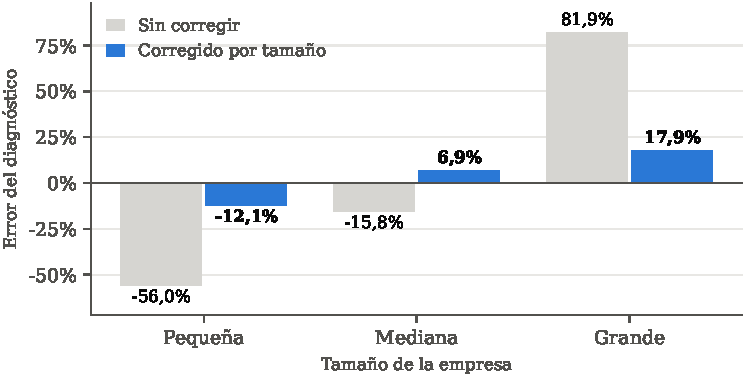
\includegraphics[width=\textwidth]{sesgo_tamano.pdf}
\vspace{1mm}
{\footnotesize Rango de error del centro: de $-$56,0\,\%/$+$81,9\,\% a
$-$12,1\,\%/$+$17,9\,\%.}
\end{column}
\end{columns}
\end{frame}

% ----------------------------------------------------------------------------
\begin{frame}
\frametitle{Cobertura, artefacto y alcance de lo reportado}
\begin{columns}[T]
\begin{column}{0.47\textwidth}
\small
\begin{tabular*}{\textwidth}{@{\extracolsep\fill}lr}
\toprule
\multicolumn{2}{l}{\textbf{Cobertura}} \\
\midrule
Techo de la etiqueta cruda & 66,6\,\% \\
Directa, sin consolidar & 57,7\,\% \\
Directa, consolidada & 64,1\,\% \\
Títulos fuera de la base & 35,9\,\% \\
\bottomrule
\end{tabular*}
\end{column}
\begin{column}{0.47\textwidth}
\small
\begin{tabular*}{\textwidth}{@{\extracolsep\fill}lr}
\toprule
\multicolumn{2}{l}{\textbf{Artefacto}} \\
\midrule
Títulos en la base & 65.181 \\
Celdas tras consolidar & 50.420 \\
Empresas con datos & 6.722 \\
Resolubles por RUC & 221.754 \\
Decisiones con evidencia & 31 \\
\bottomrule
\end{tabular*}
\end{column}
\end{columns}
\vspace{3mm}
\begin{itemize}
\item El efecto empleador acota el alcance: lo estimado es el \textbf{mercado},
no la política salarial de una empresa concreta.
\item Todo lo reportado procede de particiones de validación dentro del ajuste.
Es consistencia interna, no validación externa: el 20\,\% de evaluación final
sigue intacto.
\end{itemize}
\end{frame}

\lastslide

\end{document}
